\documentclass[letterpaper,11pt]{article}
\usepackage[spanish]{babel}
\usepackage{graphicx}
\usepackage{url}
\usepackage[utf8]{inputenc}
\usepackage{listings}
\usepackage{longtable}
\usepackage{caption}
\usepackage{algorithmic}
\usepackage{caption}
\setlength{\parindent}{1em}

\begin{document}

\begin{figure}[htp]
  \centering
  
\includegraphics[scale=0.1]{logoUSB.png}
\end{figure}

\begin{center}
  \textbf{UNIVERSIDAD SIM\'ON BOL\'IVAR}\\
  Ingenier\'ia de la Computaci\'on\\
  Dise\~no de Algoritmos II - CI-5652
\end{center}
\begin{center}	
  \vspace{2in}
  \textsf{\begin{Large}\bf One-Dimensional Cutting Stock Problem (CSP)\end{Large}}

\begin{Large}
1ra. Entrega
\end{Large}
      
\end{center}
\begin{center}
  \vspace{2in}
  Juan Garc\'ia 05-38207\\
  Federico Flaviani 99-31744\\
  \vspace{0.25in}	
  \today
\end{center}
\newpage

\tableofcontents
\newpage

\section{Introducci\'on}

\subsection{Breve descripci\'on del problema}

Cutting Stock Problem (CSP) o Problema de Corte y Empaquetamiento es un problema de optimizaci\'on
orientado al \'area de la programaci\'on entera, en donde el objetivo es minimizar el desperdicio generado
al cortar una serie de patrones en un \'area dada. Este problema surge regularmente en el \'area de la
industria sider\'urgica o del papel, en donde se busca disminuir las p\'erdidas monetarias por desperdicios
de material.\\

\begin{figure}[htp]
\centering
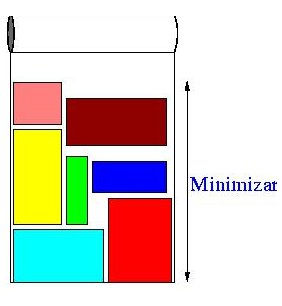
\includegraphics[scale=0.7]{faixa3.jpg}
\caption{Forma general de CSP en dos dimensiones}
\end{figure}

En CSP se dispone de un \'area la cual deseamos cortar y existen muchas maneras de representarla. Puede
ser una tela de tamaño finito en todos los sentidos, o una tela de ancho fijo con altura infinita, que es
el caso que trataremos en este proyecto. Luego se tienen una serie de formas o patrones que queremos cortar
de la mencionada tela. Dado que nuestro problema es la versi\'on unidimensional (Figura 2), las piezas que se quieren
cortar de la tela seran rectangulos con base constante igual a uno y con alturas variadas. Adem\'as no se
permitir\'a el cambio de orientaci\'on de las piezas. Instancias del problema con mas nivel de dificultad
se encuentra con la versi\'on de dos dimensiones y piezas de tamaño y formas variables, asi como en tres
dimensiones, en donde el problema se basa en optimizar la forma de empaquetar piezas en un volumen
dado, tipo un contenedor de mercancia.

\begin{figure}[htp]
\centering
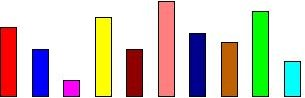
\includegraphics[scale=0.7]{Untitled.jpg}
\caption{Generalizaci\'on a cortes unidimensionales}
\end{figure}

\newpage

\section{Dise\~no}

\subsection{Modelo utilizado para representar el problema}

Como se mencion\'o anteriormente la forma en que representamos el problema es usando una tela "infinita" con
ancho fijo. Para representar la infinitud de la tela hallamos una cota superior que cubra todos los posibles
cortes que se pueden realizar, de esta forma nuestra cota superior $CS$ sera: $$ CS =  \sum_{i = 1}^{N} L_i $$ 
donde $N$ es el n\'umero de piezas a cortar y $L_i$ es el largo de la pieza $i$.\\
En nuestro programa crearemos una serie de estructuras para representar cada parte del problema, comenzando con las
piezas que queremos cortar, pasando por patrones de corte ya establecidos, los cuales representaran en
nuestro caso una soluci\'on factible.

\subsection{Estructuras y algoritmos involucrados en la aplicaci\'on}

Dentro de las principales estructuras que utilizamos, estan aquellas que nos permiten representar
un estado o soluci\'on factible. Para ellos necesitamos piezas y un patr\'on de corte, por lo tanto
se definir\'an las estrucutras \emph{Piece} y \emph{Pattern} en conjunto con su tanda de atributos
y diferentes m\'etodos.\\

En cuanto a los algoritmos utilizados, encontramos en primera instancia un algoritmo greedy que nos
permitira crear una soluci\'on inicial. Luego se aplicar\'an una serie de procedimientos con el fin de
determinar una vecindad en un cierto espacio. Para finalmente aplicar los algortimos de las diferentes
meta-heuristicas que se van a aplicar para resolver el problema.\\

El algoritmo greedy para generar una soluci\'on inicial consiste en ir aplicando cortes sucecivos a la tela, de la
manera mas eficiciente posible. Primero se ordenan los cortes a realizar seg\'un el tamaño de mayor a menor.
Se comenzar\'a por la base he iremos colocando las piezas por fila. Existir\'a un \'indice que llevar\'a la informaci\'on
de la altura lograda de menor valor, esto con el fin de comenzar una nueva tanda de corte por fila a la m\'inima
altura posible, sin tener que recorrer toda la matriz para insertar un corte. Finalmente cuando el algoritmo termina,
nos entregar\'a una dispocisi\'on de cortes donde las piezas mas grandes estan en la parte inferior, y las mas pequeñas
en el tope de la tela.

\subsubsection{Clase Piece}

Esta clase representa una pieza a ser cortada de la tela. Posee dos atributos, \emph{large} que representa
el largo del rectangulo a cortar y \emph{pos} que permite conocer la posici\'on de la pieza cortada en la
tela total. Adem\'as, como todo objeto tiene un constructor que recibe como par\'ametros un entero que representa
el largo del bloque y un arreglo bidimensional para inicializar la posici\'on del mismo en la tela.
Finalmente posee un m\'etodo \emph{clone} que permite crear una copia de una pieza.

\begin{verbatim}
class Piece {
 public:
  int large;
  int pos[2][2];
  Piece(int, int[2][2]);
  Piece clone();
};
\end{verbatim}

\subsubsection{Clase Pattern}

La clase \emph{Pattern} representa un patr\'on de corte de una isntancia del problema del CSP. Es decir es
una solucion factible, en donde estan posicionadas todas las piezas de corte sobre la tela. A partir de una
instancia de patter se obtienen otras instancias de la misma aplicacando los operadores de vecindad, asi como
se puede obtener el nivel de calidad de la misma, para hacer comparaciones entre un patr\'on y otro.\\

La clase tiene una serie de atributos y m\'etodos, pero dentro de los mas importantes encontramos a \emph{width} y
\emph{height} que representan el alto y ancho de la tela a cortar. \emph{num\_pieces} y \emph{pieces} son el n\'umero
de piezas y la lista que contiene a las mismas, repectivamente. Adem\'as otros atributos que modelan el area ocupada
y \'area libre, el n\'umero de lineas concretadas en el patr\'on y variables enteras que soportan la generaci\'on de las
vecindades.\\

Dentro de los m\'etodos mas importantes encontramos los constructores de clase, que permiten inicializar un patr\'on cualquiera, tambi\'en el m\'etodo \emph{vicinityNext} que permite ir generando la vecindad dinamincamente, basado en
los m\'etodos \emph{vicinityFirstLevel}, \emph{vicinitySecondLevel} y \emph{vicinityThirdLevel}, el m\'etodo \emph{perturbar} que permite pertubar una soluci\'on iniciada para aplicar la metaheuristica \emph{ILS}, entre otros m\'etodos de apoyo para hacer revision de calidad y de la funci\'on objetivo.

\begin{verbatim}
class Pattern {
 public:
  int width;
  int height;
  int num_pieces;
  list<Piece>* pieces;
  int area_ocup;
  int area_no_ocup;
  int lines;
  int iteTermino;
  int x,y,x2,y2,x21,y21,x3,y3,x32,y32,x31,y31;
  Pattern();
  Pattern(int, int);
  Pattern(list<Piece *>, int, int);
  Pattern perturbar(Pattern);
  int quality();
  int distance(Pattern);
  Pattern clone();
  void remove(int);
  void add(int,Piece);
  Pattern vicinityFirstLevel(bool);
  Pattern vicinitySecondLevel(bool);
  Pattern vicinityThirdLevel();
  Pattern vicinityNext();
  list<Pattern> vicinity();
  void updateHeight();
\end{verbatim}

\subsection{Representaci\'on de la soluci\'on}

La soluci\'on al problema de CSP se encuentra representada mediante la clase \emph{Pattern}, en donde se encuentra 
una lista de piezas que fueron cortadas y poseen mediante la clase \emph{Piece} una serie de atributos que denotan
la posici\'on en la tela, y forman el patr\'on como fue cortada. Adem\'as podemos saber la altura y el n\'umero de lineas 
creadas con el corte, y analizar una funci\'on objetivo.\\

Esto es de manera general, pero la estructura que en concreto representar\'a nuestra soluci\'on se basa en un arreglo de
listas de piezas. El tamaño del arreglo viene definido por el ancho fijo de la tela a cortar, y cada una de las listas
se compone por la piezas colocadas al estilo de una pila, en la columna \emph{i} del arregla o tela. Esta representaci\'on
nos ser\'a de conveniencia al momento de realizar un movimiento para generar un estado vecino.

\subsection{Funci\'on Objetivo}

La funci\'on objetivo que vamos a utilizar esta definida por diferentes par\'ametros. De manera general definimos
una m\'etrica de calidad de los estados soluci\'on basada en la m\'axima altura generada por el corte de cada una de las piezas.
Es decir que si comparamos dos estados soluci\'on, en donde ambos tengan un patr\'on con el mismo n\'umero de piezas cortadas, 
es decir, la misma \'area ocupada, aquel patr\'on que tenga la altura menor sera la mejor. En primera instancia esa es la m\'etrica que vamos a utilizar en nuestro problema.\\

Otra funci\'on objetivo que podemos usar esta basada en el n\'umero de lineas completas generadas en el patr\'on, es decir,
todas las lineas completas de que tengan el ancho total de la tela, y como altura una unidad. El problema de esta m\'etrica es que podemos encontrar dos patrones con el mismo n\'umero de lineas, pero con alturas muy diferente, en donde el malgasto sea excesivo.\\

Una idea mejor es crear una funci\'on objetivo que relacione las dos m\'etricas anteriores, aunque actualmente no 
hemos definido esta estrategia para ser usada en las metaheuristicas a implementar.

\subsection{Operadores}

Para generar la vecindad para un estado soluci\'on utilizamos un conjunto de tres operadores, pero que pueden ser ultilizados
por separado para generar tres tipos de vecindades. Los tres operadores se basan en el moviento de piezas, el operador
de primer nivel genera una vecindad moviendo una pieza selecciona de los niveles superiores. El siguiente operador, de segundo nivel, fija una pieza seleccionada y realiza una llamada recursiva al operador de primer nivel, al final se recolocar\'a la pieza fijada, resultando asi un movimiento de dos piezas. El tercer operador es una llamada al operador de
tercer nivel, en donde se fija una pieza y se llama a el operador de segundo nivel.

\newpage

\section{Detalles de implementaci\'on}

\subsection{Pseudocodigo de las estructuras}

\subsubsection{Algoritmo de Local Search}

\subsubsection{Algoritmo de Colonia de Hormigas}

Para entender el algoritmo de hormigas que hemos implementado restringiremos la altura maxima 
que nuestros patrones pueden tener por $L$ fijo y seguidamente indexemos el conjunto de las piezas de $1$ hasta $n$, 
con $n$ igual al total de piezas distintas:

\begin{definicion}
Definiremos las variables $l_i$ como la longitud de la pieza $i$
\end{definicion}

\begin{definicion}
Una columna factible es un multiconjunto de enteros $\{i_1 ,i_2 ,\dots ,i_h\}$ tales que $\Sigma _{k=1}^h l_{i_k}\leq L$.
\end{definicion}

Dado un numero de tipos de piezas fijas y sus respectivas longitudes, se tiene que el n\'umero 
total de columnas factibles es finito, denotemos a este n\'umero finito por $m$ e indexemos el conjunto de columnas 
factibles.

\begin{definition}
Sea $\{i_1 ,i_2,\dots ,i_h\}$ la columna factible $j$, denotemos entonces por $S_i$ como el n\'umero $L-\Sigma _{k=1}^h l_{i_k}$ 
y a $O_{ij}$ como la cantidad de veces que se repite el entero $i$ en la columna factible $j$ 
\end{definition}

A continuaci\'on describiremos el algoritmo:

El concepto de columna factible es fundamental para nuestro algoritmo de hormigas, por lo tanto es importante destacar que representaremos 
una columna factible $j$ como un arreglo de enteros de tama\~no igual al total de piezas distintas y donde cada entero 
ser\'a un $O_{ij}$.

La primera etapa del algoritmo consiste en calcular todas las posibles columnas factibles y colocar cada una de ella en un 
arreglo, de modo que este arreglo implementa la indexaci\'on necesaria que se mensionaba en los p\'arrafos anteriores para poder definir 
las variables $S_j$ y $O_{ij}$.

La idea del algoritmo es que en cada iteraci\'on, cada hormiga escoja probabilisticamente una columna factible hasta el punto que el 
total de las piezas de todas estas columnas sobrepase el total de las piezas del problema. El exeso de piezas ser\'a penalizado en la 
funci\'on objetivo y las probabilidades de escogencia de columna ser\'a menor en la medida que de estas escogencias resulte un crecimiento del n\'umero 
extras de piezas.

La funci\'on objetivo seg\'un lo dicho anteriormente ser\'a $\Sigma _{j=1}^m S_jX_j+\Sigma _{i=1}^n V_i$ donde $X_i$ es el n\'umero de veces 
que se us\'o la columna factible $j$ en la soluci\'on y $V_i$ es el total de las piezas extras.

Las probabilidades de escogencia de las columnas se realizan en dos etapas: Primero se escoje una pieza probabilisticamente y luego se escoje 
(probabilisticamente tambien) una columna donde se encuentre la pieza escojida. 

\begin{algorithmic}

\REQUIRE Patron inicial : actual

\STATE $k \gets 0$
\STATE Patron next
\WHILE{ $k < 100 \quad \wedge \quad !actual.iteTermino$} 
	\WHILE{ $k < 100 \quad \wedge \quad !actual.iteTermino$} 
		\STATE $next  \gets actual.vicinityNext()$
		\IF {$next \neq NULL \quad \wedge \quad next.quality() < actual.quality()$}
        	\STATE $actual.destroy()$
          	\STATE $actual \gets next$
          	\STATE k++
	    \ELSE
        	\STATE $next.destroy()$
      	\ENDIF
    \ENDWHILE
\ENDWHILE

\RETURN actual

\end{algorithmic}

\subsubsection{Algoritmo de Local Search - Mejor Mejor}

\begin{algorithmic}

\REQUIRE Patron inicial: actual

\STATE $k \gets 0$
\STATE Patron next
\STATE Patron best
\STATE $best \gets actual$

\WHILE {$ k < 100 $}
	\WHILE {$!actual.iteTermino$}
 		\STATE $next \gets actual.vicinityNext()$
		\IF {$next \neq NULL \quad \wedge \quad next.quality() < actual.quality()$}
        	\STATE $best \gets next$
        \ELSE
        	\STATE $next.destroy()$
    	\ENDIF
    \ENDWHILE
	\IF {$actual = best$}
      	\STATE break
    \ELSE
      	\STATE $actual \gets best$
  	\ENDIF
  	\STATE k++
\ENDWHILE
\RETURN actual

\end{algorithmic}

\subsubsection{Algoritmo de ILS}

\begin{center}
\begin{algorithmic}

\REQUIRE Patron inicial: $s_{mejor}$

\STATE $k \gets 0$
\STATE $s_{mejor} \gets localSearch(s_{mejor})$

\WHILE {$ k < 100 $}
	\STATE Patron s1
    \STATE $ s1 \gets s_{mejor}.perturbar() $
    \STATE $ s1 \gets localSearch(s1) $
    \IF {$ s1.quality() < s_{mejor}.quality()$ }
    	\STATE $ s_{mejor}.destroy() $
        \STATE $ s_{mejor} \gets s1 $
    \ELSE
    	\STATE $ s1.destroy() $
        \STATE break
    \ENDIF
    \STATE k++
\ENDWHILE
\RETURN $s_{mejor}$

\end{algorithmic}
\end{center}

\newpage

\section{Instrucciones de operaci\'on}

Para compilar el programa debe realizar la llamada:
\begin{verbatim}
    $> make
\end{verbatim}
Y para realizar la corrida:
\begin{verbatim}
    $> ./CSP
\end{verbatim}

\section{Estado actual}

\subsection{Estado final de la aplicaci\'on}

La aplicaci\'on no se encuentra del todo operativa, sin embargo fue posible implementar
el algoritmo greedy para generar la soluci\'on inicial, los operadores mencionados
anteriormente para generar la vecindad, y las metaheur\'isticas de Local Search,
Local Search con Mejor-Mejor e ILS.

\subsection{Errores}

Existe un problema en la implementaci\'on de las metaheur\'isticas que no permite salir de
los \'optimos locales que se encuentra en la soluci\'on greedy inicial. Esto es para casos,
en que los movimientos que deban realizarse sean mas de cuatro. B\'asicamente hace falta
un operador que logre concretar movimientos a mas de cuatro niveles, o que gracias a las
sugerencias de los compañeros en el aula, se logre realizar una perturbaci\'on mayor a la
instancia, para asi llegar de otra manera al optimo global.

\newpage

\section{Conclusiones y recomendaciones}

Durante el desarrollo de esta primera entrega, pudimos notar el nivel de dificultad que posee este problema,
sobre todo para encontrar una representaci\'on ideal. \'Ademas en la literatura existen una gran cantidad de
variaciones del mismo, lo que a veces puede resultar en una complicaci\'on al momento de definir las bases
para nuestro problema espec\'ifico.\\

Sin embargo fue posible realizar una implementaci\'on que logre representar efectivamente nuestro problema, y 
a partir de alli utilizar algunas metaher\'isticas para encontrar una buena soluci\'on al mismo. Aunque dado a las
complicaciones generadas no fue posible realizar un an\'alisis exaustivo de las metaheur\'isticas.

\subsection{Mejoras}

Es necesario mejorar nuestros operadores de vecindad, dado que en estos momentos se esta creando una vecindad
muy grande, y que no permite hallar una buena soluci\'on. Con recomendaciones de los colegas en la disciplina y
la profesora, se proceder\'a a mejorar nuestros operadores de vecindad, y ademas aplicar las metaheur\'isticas con
tendencia probabilisticas, las cuales deberian ayudar a mejorar las soluciones obtenidas hasta ahora.

\newpage

\section{Tablas}

\begin{center}
\begin{longtable}{|c|c|}
\hline
Parametro & Valor \\
\hline
 k = Nro. iteraciones LS & 100 \\
\hline
 k = Nro. iteraciones LS Mejor-Mejor & 100 \\
\hline
 k = Nro. iteraciones ILS & 100 \\
\hline

\caption{Parametros}
\end{longtable}
\end{center}

La instancia que se presenta a continuacion tenia 66 piezas, y la solucion inicial tenia como funcion
de calidad 20.

\begin{center}
\begin{longtable}{|c|c|c|}
\hline
Heuristica & Optimo Alcanzado & Tiempo (seg) \\
\hline
 Local Search & 4 & 6.616 \\
\hline
 LS Mejor-Mejor & 4 & 17.558 \\
\hline
 ILS & 4 & 12.370 \\
\hline

\caption{Tiempo de las heuristicas para instancia de 66 piezas}
\end{longtable}
\end{center}

\newpage

\section{Referencias bibliogr\'aficas}

\begin{thebibliography}{99}
  
\bibitem[1]{ref:steel}
  \textbf{Solving the Cutting Stock Problem in the Steel Industry}\\
  \textit{KARELAHTI J.}

\bibitem[2]{ref:genetic}
  \textbf{A Genetic Solution for the Cutting Stock Problem}\\
  \textit{ANDRAS P., ANDRAS A, SZABO Z.}

\bibitem[3]{ref:prog}
  \textbf{A Progressive Heuristic Search for the Cutting Stock Problem}\\
  \textit{ONAINDIA E., BARBER F., BOTTI V., CARRASCOSA C., HERNANDEZ M., REBOLLO M.}
  
\end{thebibliography}
  
\end{document}
